\section{Experiments on Image Source Separation}
\subsection{Software requirements}
The software in this project has prerequisite on several opensource Matlab Toolboxes (i.e. WaveLab 850, K-SVD, MCALab110 and image processing toolbox). Complete version of my code can be found on Github\footnote{https://github.com/Dieselmarble/FYP}. In addition, I wrote my own BS-KSVD Toolbox which involves some novelty.

\subsection{Solve the BSS scale and permutation indeterminacy}
As mentioned in previous sections, BSS methods suffers from ambiguities that the estimated source can be scaled permuted up to any arbitrary order. The solution to this problem is equivalent to an optimal assignment algorithm. An intuitive methods would be comparing the similarity metric (e.g. Euclidean distance) between every estimated source and the original sources. It is easy to see that the complexity is $O(n^2)$. Unfortunately, the optimal assignment may not, in general, be attained in this way \cite{1261953}. In this report, we employ the Kuhn-Munkres Algorithm (also well-known as the Hungarian Algorithm)
with a higher complexity $O(n^3)$ (n is the number of channels) but guarantees the optimal assignment to calculate the permutation matrix.

\subsection{Image Decomposition}
In this section, we turn to use MMCA to separate two-dimensional data and compare the result with the standard ICA source separation techniques. \\

In Figure (\ref{segmentation_Im} a) are two source signals, one of which is oscillating textures while another is  a `boy' image. Curvelet transform is selected as the dictionary for source 1 and discrete consine transform is selected for source 2. This is similar to adpot the idea of a double sparse dictionary therefore we can decompose the mixtures into cartoon and texture. Figure (\ref{segmentation_Im} c) illustrates the separated image using MCA under the presence of 20dB Gaussian noise. It can be shown that MCA is able to split the texture and cartoon parts. However, the reconstruction quality of the `boy' image using curvelet dictionary in MCA does not give satisfactory result though. We think the decomposition presenting in the dictionary domain may not be extremely sparse, as some of the mixtures can still be seen in the output image. \\

Note that the MCA algorithm, unlike BSS methods, only takes one single combination of sources ($m = 1$). Now we extend the observed mixtures to a multichannel case and BSS techniques applies. The correlation coefficient between two sources are only 0.07. Hence the independence assumption for ICA methods is valid here. We create four mixtures from two source images.
\ref{segmentation_Im} (d) shows that MMCA is clearly able to efficiently separate the original source images, achieving better visual results than FastICA in (b). Quantitatively, Figure \ref{segmen_1} shows the correlation between the original sources and those estimated. As the data noise variance increase, 
MMCA (dashed line) clearly achieves better estimation quality and shows clear robustness compared to non de-noised ICA methods. In addition, one can note that both JADE and FastICA provides similar performance.\\

Figure \ref{segmen_1} plots the matrix estimation error is defined as $||\mathbf{I_n} - P\tilde{\mathbf{A}}^{+}\mathbf{A} ||$, after elimination the effect of the permutation and scale indeterminacy. Contrasting with standard ICA methods, MMCA iteratively estimates the mixing matrix from coarse (i.e., smooth) versions of the sources and thus is not penalized by the presence of noise. As a consequence, MMCA is clearly more robust to noise than standard ICA methods, even under very noisy context \cite{BobinJ_2006Mdas}. This result reflects our expectation in section \ref{ica_defect} that ICA is not robust under the additive Gaussian nosie setting.\\

The results in this experiment proves that sparsity based methods successfully handle the image segmentation task. Especially under the multichannel case, MMCA significantly outperforms the standard ICA methods in terms of separation quality and robustness.\\




% -------------------------
\begin{figure}[!htbp]
\centering
\subfigure[]{
\begin{minipage}[b]{0.23\linewidth}
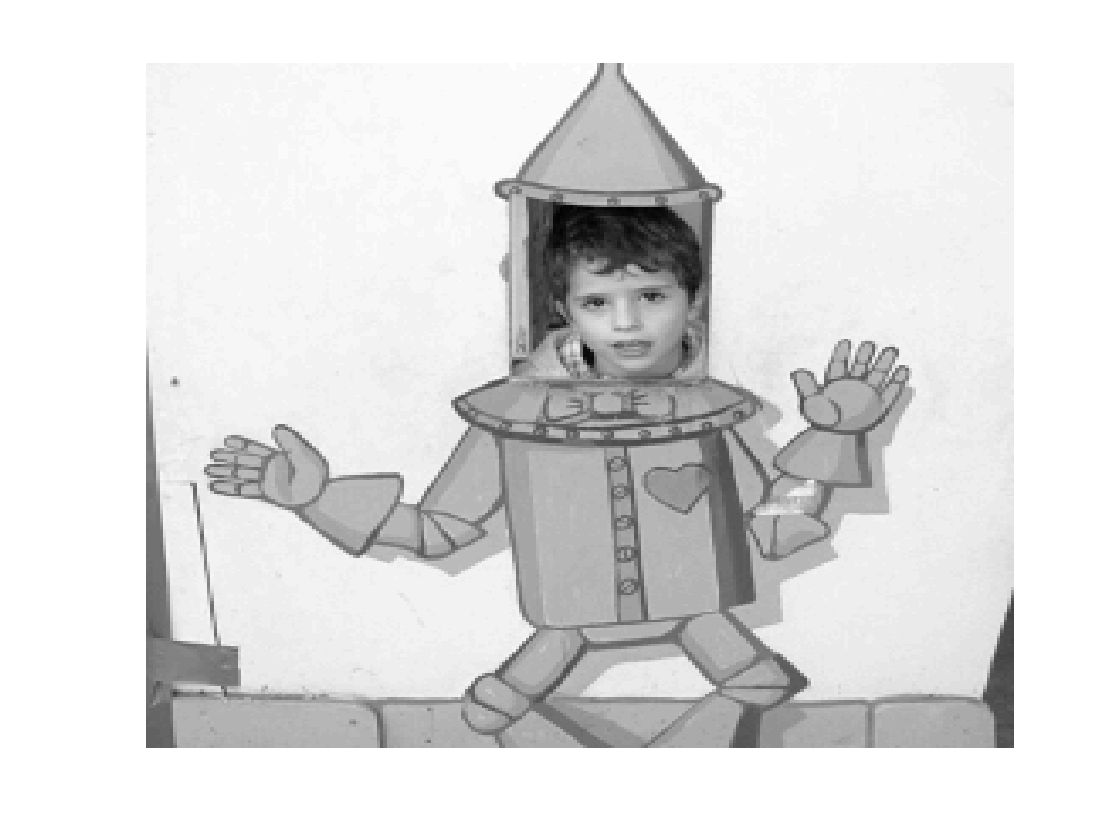
\includegraphics[width=1\linewidth]{images/source1.png}\vspace{1pt}
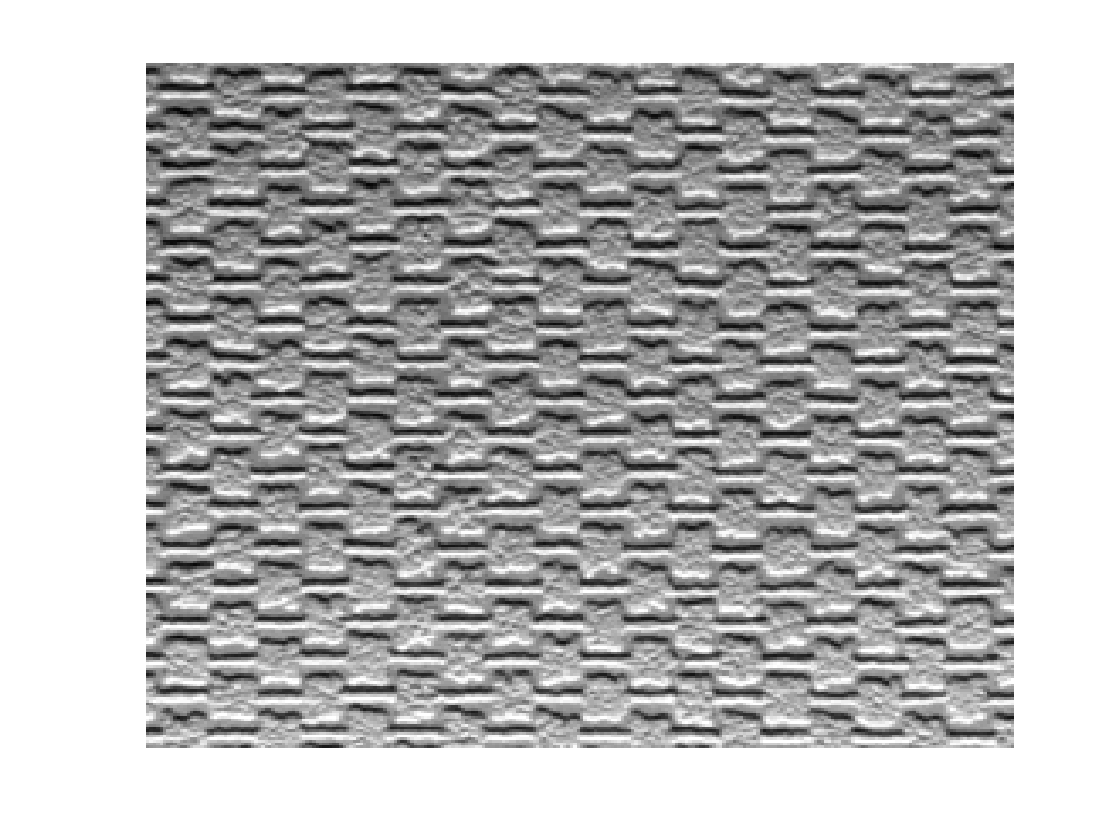
\includegraphics[width=1\linewidth]{images/source2.png}
\end{minipage}}
\subfigure[]{
\begin{minipage}[b]{0.23\linewidth}
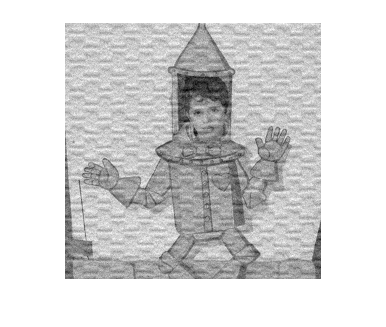
\includegraphics[width=1\linewidth]{images/separated1.png}\vspace{1pt}
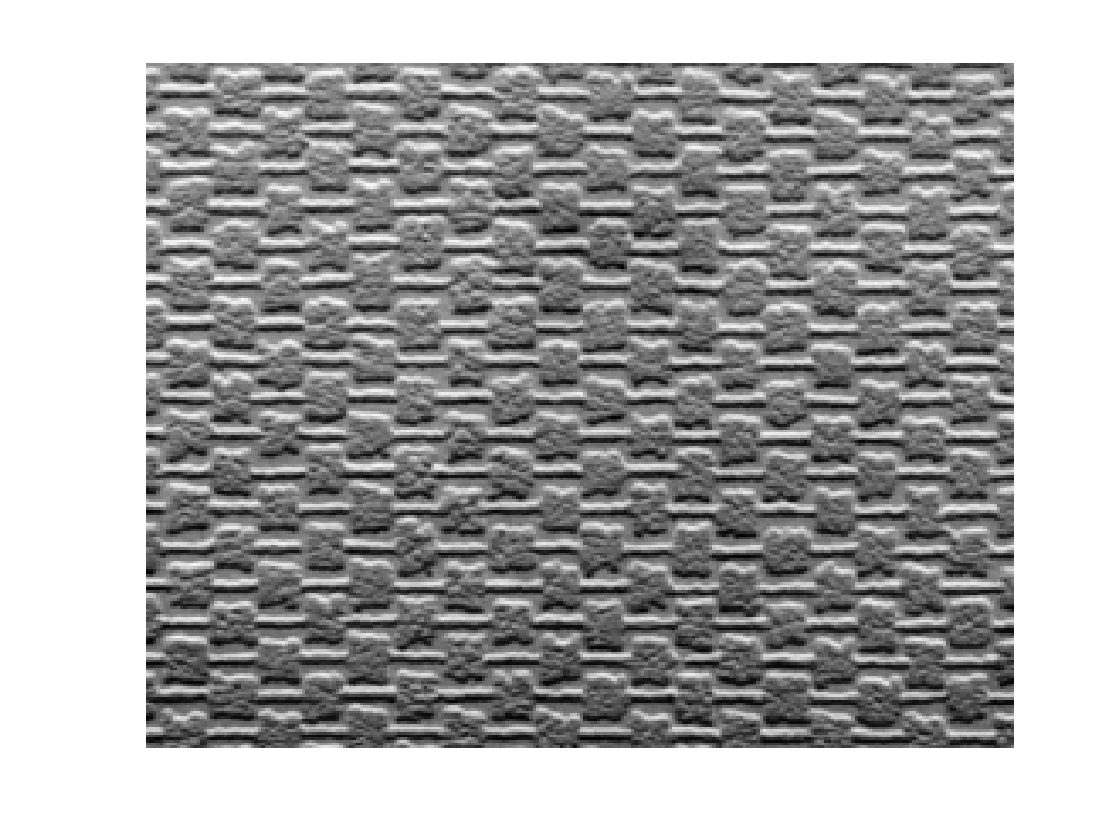
\includegraphics[width=1\linewidth]{images/separated2.png}
\end{minipage}}
\subfigure[]{
\begin{minipage}[b]{0.23\linewidth}
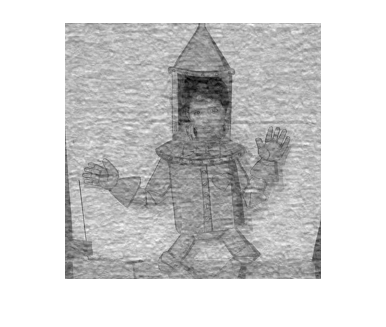
\includegraphics[width=1\linewidth]{images/MCA_Cartoon.png}\vspace{1pt}
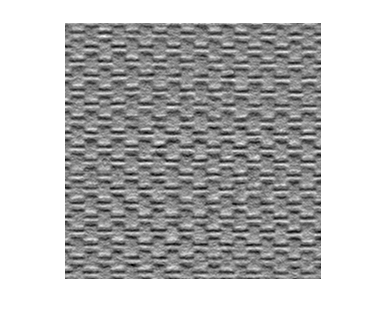
\includegraphics[width=1\linewidth]{images/MCA_Texture.png}
\end{minipage}} 
\subfigure[]{
\begin{minipage}[b]{0.23\linewidth}
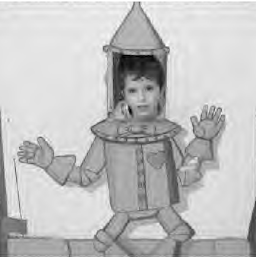
\includegraphics[width=1\linewidth]{images/mmca_cartoon.png}\vspace{1pt}
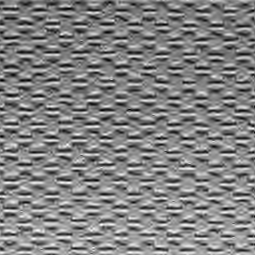
\includegraphics[width=1\linewidth]{images/mmca_texture.png}
\end{minipage}}
\caption{Experiment1: Image segmentation (PSNR = 20dB); \textbf{(a)}: Original sources; \textbf{(b)}: FastICA outputs; \textbf{(c)}: MCA outputs; \textbf{(d)}: MMCA outputs}
\label{segmentation_Im}
\end{figure}
% -------------------------


\begin{figure}[!htbp]
\centering
\begin{minipage}[b]{0.49\textwidth}
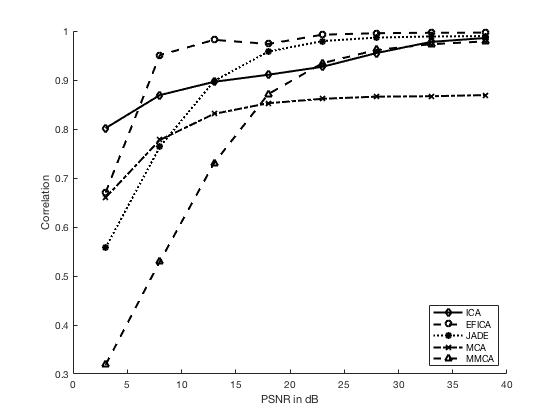
\includegraphics[width=\textwidth]{images/corr_plot_seg.png}
\caption{Evolution of the correlation coefficient between original and estimated sources as the noise variance varies.}
\label{segmen_1}
\end{minipage}
\begin{minipage}[b]{0.49\textwidth}
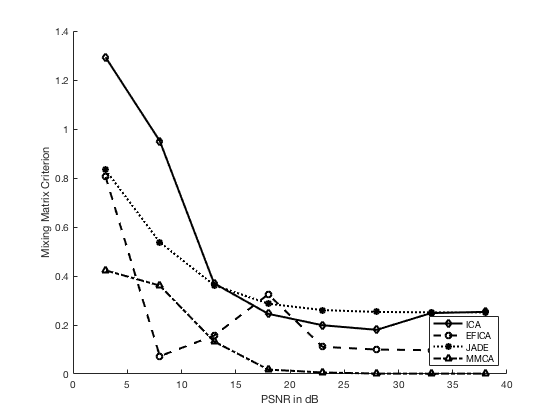
\includegraphics[width=\textwidth]{images/mmc_plot_seg.png}
\caption{Evolution of the mixing matrix criterion (after indeterminacy corrected) as the noise variance varies.}
\end{minipage}
\label{segmen_2}
\label{imapint1}
\end{figure}

\newpage
\subsection{Blind Image Source Separation}
In this experiment, we mix 4 pictures into 10 channels. The source images are picked as they contains similar morphologies. Classical ICA methods and MMCA, GMCA are applied to separate the source. Unfortunately the FastICA methods is not able to separate the original source. We hence adopt a sophisticated variant of it abbreviated as EFICA. Moreover, it has been proved in \cite{BobinJ_2007SaMD} that using a single overcomplete DWT dictionary or a union of DCT and DWT dictionary in GMCA provides similar results. We therefore use a discrete wavelet dictionary in FastGMCA (FGMCA).\\


GMCA has been proved elsewhere \cite{BobinJ_2007SaMD} that it achieves better separation quality when the estimated components are 'very' sparse in the given dictionary. Therefore GMCA is supposed to perform well on separating images even without distinct discrepancies. Separated images are displayed in Figure (\ref{BSS_ex2_11}). It shows the recovered image by various BSS methods contaminated by 20dB noise. All methods can distinguish the barbara image (row 3) from the mixtures. The ICA methods, nonetheless fail to separate the scenery photos (row 1 and 2). But in (e) using GMCA still gives acceptable result. MMCA using curvelet + DCT in (d) gives better result than ICA methods, but not so good as GMCA.\\


% ---------- begin figure-------------
\begin{figure}[!htbp]
\centering
\subfigure[]{
\begin{minipage}[b]{0.17\linewidth}
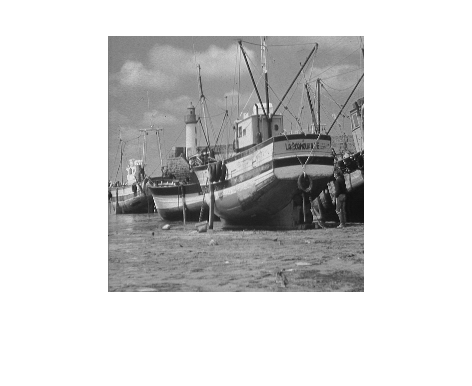
\includegraphics[width=1\linewidth]{images/boat_ori.png}\vspace{4pt}
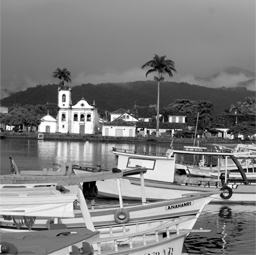
\includegraphics[width=1\linewidth]{images/paraty_ori.png}\vspace{4pt}
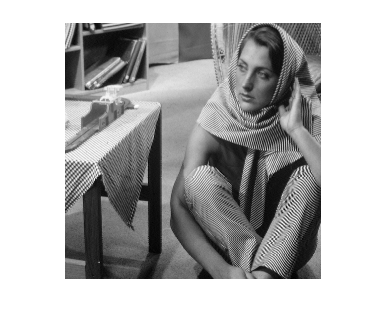
\includegraphics[width=1\linewidth]{images/barbara_ori.png}\vspace{4pt}
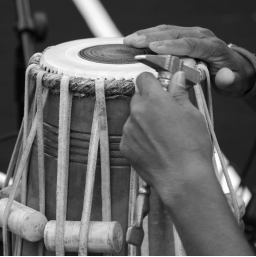
\includegraphics[width=1\linewidth]{images/pakhawaj_ori.png}
\end{minipage}}
\subfigure[]{
\begin{minipage}[b]{0.17\linewidth}
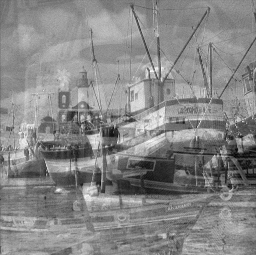
\includegraphics[width=1\linewidth]{images/efica_out1.png}\vspace{4pt}
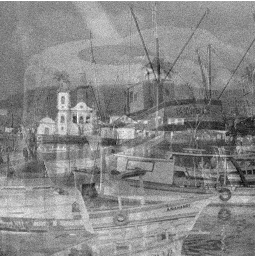
\includegraphics[width=1\linewidth]{images/efica_out2.png}\vspace{4pt}
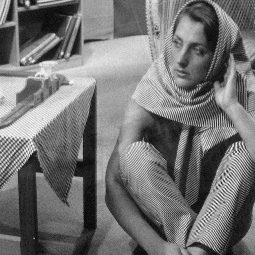
\includegraphics[width=1\linewidth]{images/efica_out3.png}\vspace{4pt}
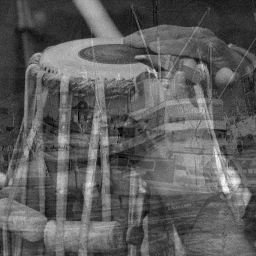
\includegraphics[width=1\linewidth]{images/efica_out4.png}
\end{minipage}}
\subfigure[]{
\begin{minipage}[b]{0.17\linewidth}
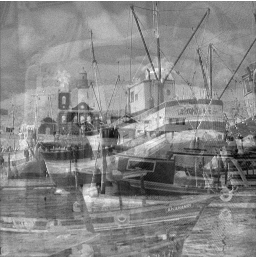
\includegraphics[width=1\linewidth]{images/jade_out1.png}\vspace{4pt}
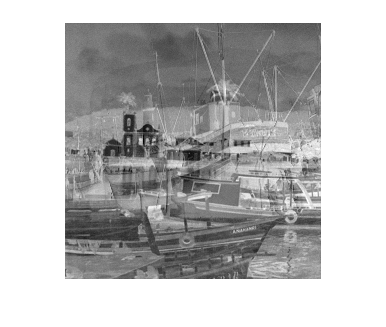
\includegraphics[width=1\linewidth]{images/jade_out2.png}\vspace{4pt}
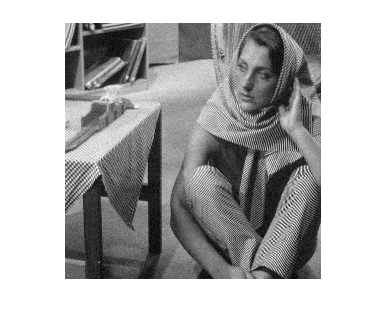
\includegraphics[width=1\linewidth]{images/jade_out3.png}\vspace{4pt}
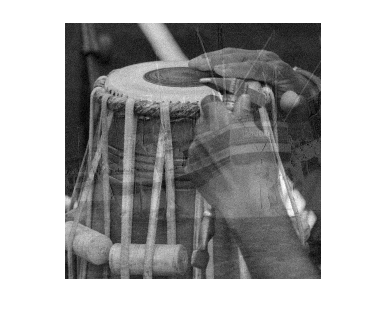
\includegraphics[width=1\linewidth]{images/jade_out4.png}
\end{minipage}}
\subfigure[]{
\begin{minipage}[b]{0.17\linewidth}
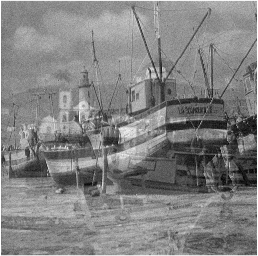
\includegraphics[width=1\linewidth]{images/mmca_ex24.png}\vspace{4pt}
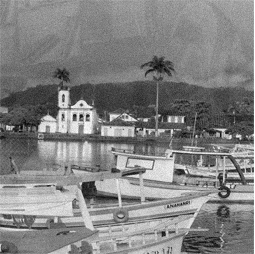
\includegraphics[width=1\linewidth]{images/mmca_ex22.png}\vspace{4pt}
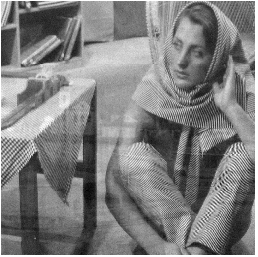
\includegraphics[width=1\linewidth]{images/mmcaex21.png}\vspace{4pt}
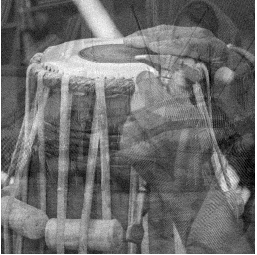
\includegraphics[width=1\linewidth]{images/mmca_ex23.png}
\end{minipage}}
\subfigure[]{
\begin{minipage}[b]{0.17\linewidth}
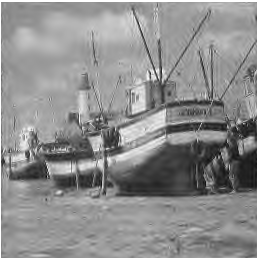
\includegraphics[width=1\linewidth]{images/gmca_out1.png}\vspace{4pt}
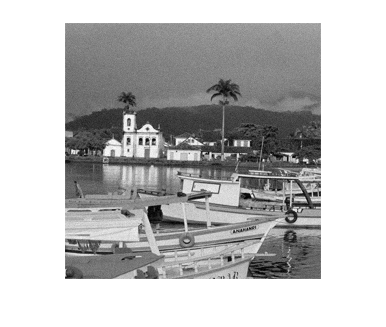
\includegraphics[width=1\linewidth]{images/gmca_out2.png}\vspace{4pt}
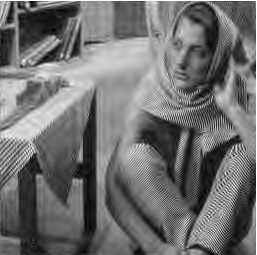
\includegraphics[width=1\linewidth]{images/gmca_out3.png}\vspace{4pt}
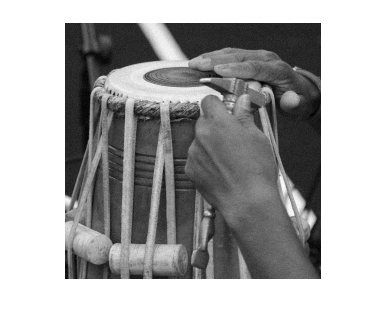
\includegraphics[width=1\linewidth]{images/gmca_out4.png}
\end{minipage}}
\caption{Experiment2: image separation (20dB noise); \textbf{(a)}:Original image sources; \textbf{(b)}:EFICA outputs; \textbf{(c)}:JADE outputs; \textbf{(d)}:MMCA outputs; \textbf{(2)}:GMCA outputs.}
\label{BSS_ex2_11}
\end{figure}

% ----------end figure------------- %

Figure (\ref{BSS_EV21}) portrays the evolution of average correlation coefficient over 4 estimated sources as a funciion of the noise variance. At a first glance, GMCA significantly outperforms the ICA methods interms of robustness and separation quality. JADE performs the worst in among all ICA based algorithms. Figure (\ref{BSS_EV21}) depicts the behavior of the imxing matrix criterion as the noise decreases. The mixing matrix criterion also clearly revels the strength of GMCA method.\\

% ----------begin figure------------- %
\begin{figure}[!htbp]
\centering
\begin{minipage}[b]{0.49\textwidth}
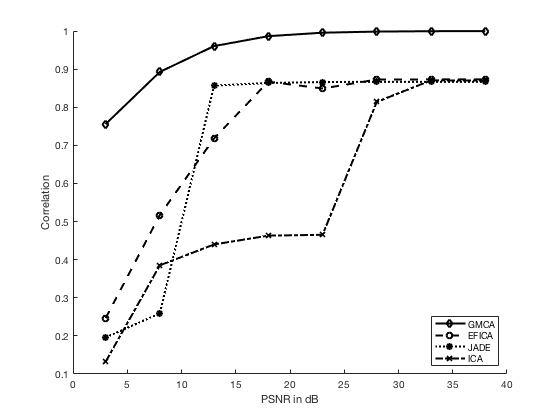
\includegraphics[width=\textwidth]{images/image_separation1.png}
\caption{Evolution of the correlation coefficient between original and estimated sources as the noise variance varies.}
\label{BSS_EV21}
\end{minipage}
\begin{minipage}[b]{0.49\textwidth}
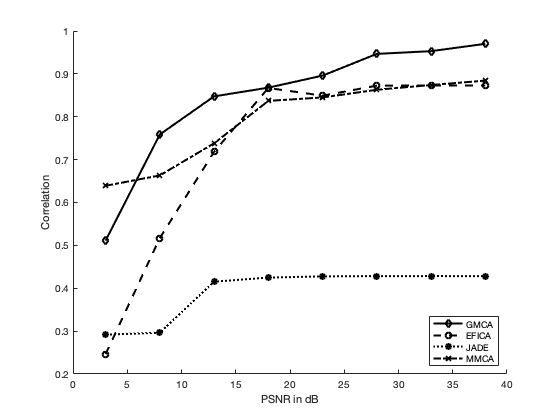
\includegraphics[width=\textwidth]{images/image_separation2.png}
\caption{Evolution of the mixing matrix criterion (after indeterminacy corrected) as the noise variance varies.}
\label{BSS_EV22}
\end{minipage}
\end{figure}
% ----------end figure------------- %

To summarise the findings in this experiment, GMCA does take good advantage of overcompleteness and morphological diversity. We can aslo claim that sparsity brings better results. Taking the advantages further, in next experiment, we explore how locally learned dictionary helps the blind source separation.\\

\subsection{Blind image separation using adaptive dictionary learning}

In this experiment, simulations are provided to demonstrate the performance of the proposed BK-SVD algorithms, as compared with the baseline algorithms, K-SVD. Same as last experiment settings, a severe case of 4 image sources with very different morphologies was chosen to exam the performance of the methods. 400 iterations were selected as the stopping criterion, addive gaussian noise is added from 3dB to 40dB. The wavelet based GMCA is selected as the baseline algorithm.\\

In order to obtain enough training samples for dictionary learning, multiple overlapped segments (patches) of the sources are taken \cite{VAbolghasemi2012}. Choose the optimal patch size is a subtle problem. Generally, very large patches should be avoided as they lead to massive dictionaries and also provide few training samples for the dictionary learning stage. We choose $8\times 8$ patches for this experiment. Furthermore the patches are $50\%$ overlapped as suggested in \cite{VAbolghasemi2012}. Maximal block size it set to be $s= 3$ and number of atoms belong to a bock is $k=2$ for BK-SVD+SAC. A standard DCT dictionary is chosen during initialisation. All dictionaries obtained have size of $64\times 256$. Consequently, each dictionary in (\ref{dictionary_learned}) have $16 \times 16 = 256$ blocks whereas each block is obtained from a $8\times 8$ patches. Figure (\ref{dictionary_learned}) also illustrates that both K-SVD and the proposed BK-SVD have good adaption to the corresponding sources, and looks significantly different from the standard DCT dictionary.\\

\begin{figure}[!htbp]
\centering
\subfigure[]{
\begin{minipage}[b]{0.99\linewidth}
\centering
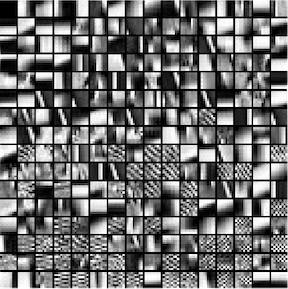
\includegraphics[width=0.15\linewidth]{images/dic1.png}\vspace{4pt}
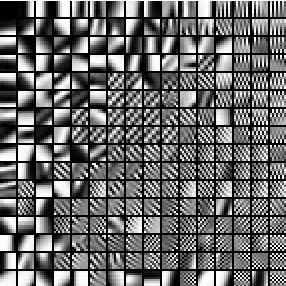
\includegraphics[width=0.15\linewidth]{images/dict3.png}\vspace{4pt}
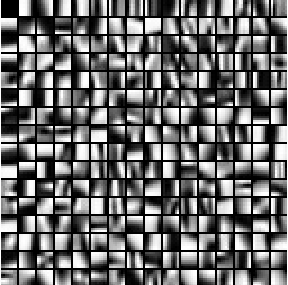
\includegraphics[width=0.15\linewidth]{images/dic2.png}\vspace{4pt}
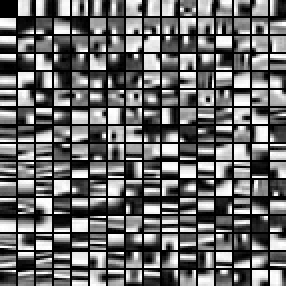
\includegraphics[width=0.15\linewidth]{images/dict4.png}
\end{minipage}}
\subfigure[]{
\begin{minipage}[b]{0.99\linewidth}
\centering
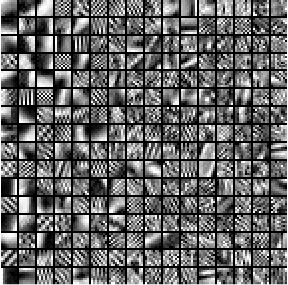
\includegraphics[width=0.15\linewidth]{images/block_dict1.png}\vspace{4pt}
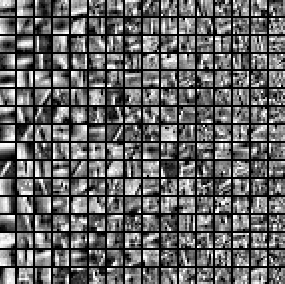
\includegraphics[width=0.15\linewidth]{images/blockdict2.png}\vspace{4pt}
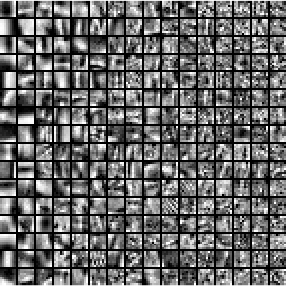
\includegraphics[width=0.15\linewidth]{images/blockdict3.png}\vspace{4pt}
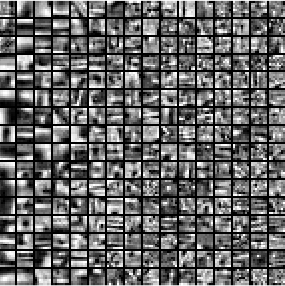
\includegraphics[width=0.15\linewidth]{images/blockdict4.png}
\end{minipage}}
% \vspace{-0.5cm} 
\caption{(a): Trained dictionary using K-SVD for sources 1,2,3,4 respectively; (b): Trained dictionary using SAC+BK-SVD for the 4 sources.}
\label{dictionary_learned}
\end{figure}

Figure (\ref{apt_compare}) visually compares the separation results
using several algorithm under 20dB Gaussian noise ($\sigma = 15$). Visually we can see that both two adaptive dictionary learning methods outperform the GMCA method in terms of recovered image quality. The learned dictionary helps to restore more details of the original iamge. Moreover, compared to the proposed methods, separated image in K-SVD+MMCA is a bit blurry. We think 400 iterations maybe too large for this problem and the 
algorithm overfits. Afterall, the proposed method will show superiority to GMCA and K-SVD+MMCA in next paragraph.\\


% ---------begin figure ------------ %
\begin{figure*}[!htbp]
\centering
\subfigure[]{
\begin{minipage}[b]{0.17\linewidth}
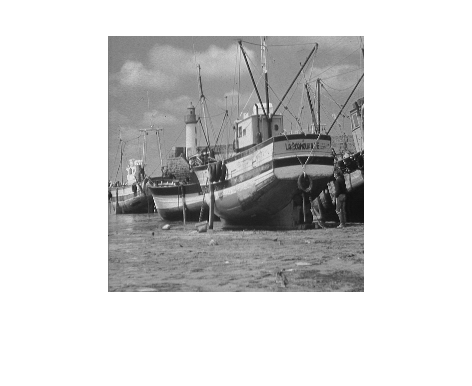
\includegraphics[width=1\linewidth]{images/boat_ori.png}\vspace{4pt}
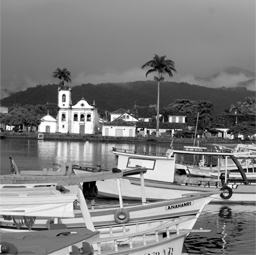
\includegraphics[width=1\linewidth]{images/paraty_ori.png}\vspace{4pt}
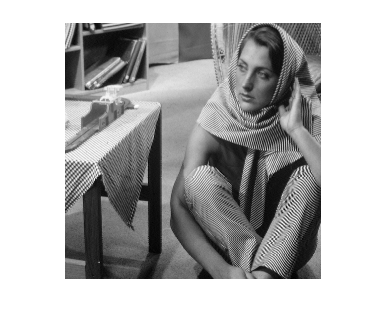
\includegraphics[width=1\linewidth]{images/barbara_ori.png}\vspace{4pt}
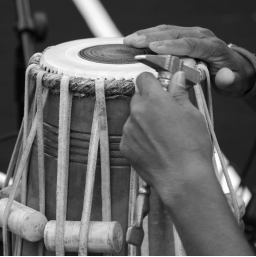
\includegraphics[width=1\linewidth]{images/pakhawaj_ori.png}
\end{minipage}}
\subfigure[]{
\begin{minipage}[b]{0.17\linewidth}
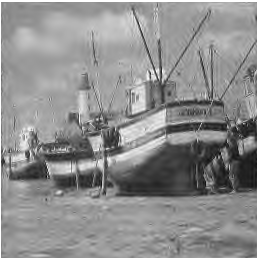
\includegraphics[width=1\linewidth]{images/gmca_out1.png}\vspace{4pt}
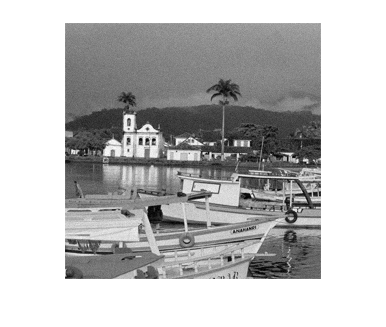
\includegraphics[width=1\linewidth]{images/gmca_out2.png}\vspace{4pt}
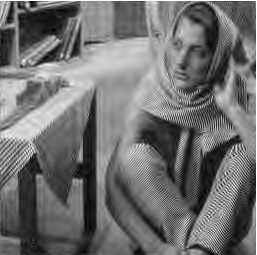
\includegraphics[width=1\linewidth]{images/gmca_out3.png}\vspace{4pt}
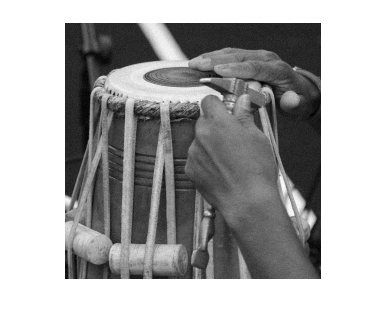
\includegraphics[width=1\linewidth]{images/gmca_out4.png}
\end{minipage}}
\subfigure[]{
\begin{minipage}[b]{0.17\linewidth}
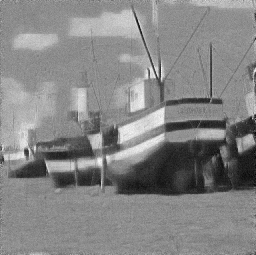
\includegraphics[width=1\linewidth]{images/ammca_out4.png}\vspace{4pt}
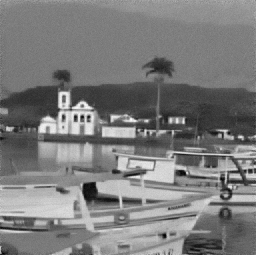
\includegraphics[width=1\linewidth]{images/ammca_out2.png}\vspace{4pt}
\includegraphics[width=1\linewidth]{images/ammca_out3.png}\vspace{4pt}
\includegraphics[width=1\linewidth]{images/ammca_out1.png}
\end{minipage}}
\subfigure[]{
\begin{minipage}[b]{0.17\linewidth}
\includegraphics[width=1\linewidth]{images/sub_bk3.png}\vspace{4pt}
\includegraphics[width=1\linewidth]{images/bk1.png}\vspace{4pt}
\includegraphics[width=1\linewidth]{images/bk2.png}\vspace{4pt}
\includegraphics[width=1\linewidth]{images/bk4.png}
\end{minipage}}
\caption{Experiment 3 (20dB noise): Using adaptive dictionary learning; \textbf{(a)}: original sources; \textbf{(b)}:GMCA outputs; \textbf{(c)}:K-SVD+MMCA output; \textbf{(d)}:BK-SVD+SAC+MMCA outputs;}
\label{apt_compare}
\end{figure*}
% ---------end figure ------------ %

We have shown via visual results that the block-structure dictionary learning algorithm provides convincing contribution to the blind source separation. Moreover, both the correlation and representation error proves our dictionary design method gives better performance. For PSNR smaller than 13dB, the proposed block-sparsifying BSS method yields similar correlation coefficient as the K-SVD method and GMCA. This is because when the SNR is low, the algorithm may no longer sucessfully build a appropriate block structure. For low noise settings (PSNR is high), the proposed method clearly outperforms the other two methods. All three methods performs well in solving the mixing matrix in low noise settings, where BK-SVD behaves slightly better. Figure (\ref{BSS_EV21_1}) plots the total reconstruction error computed as $||\mathbf{Y} - \mathbf{AX}||_2$. We can see that the proposed SAC+BK-SVD leads to smaller errors than the K-SVD method.\\


% ----------begin figure------------- %
\begin{figure}[!htbp]
\centering
\begin{minipage}[b]{0.49\textwidth}
\includegraphics[width=\textwidth]{images/adpt_plot1.png}
\caption{Evolution of the correlation coefficient between original and estimated sources as the noise variance varies.}
\label{BSS_EV21}
\end{minipage}
\begin{minipage}[b]{0.49\textwidth}
\includegraphics[width=\textwidth]{images/apt_plot2.png}
\caption{Evolution of the mixing matrix criterion (after indeterminacy corrected) as the noise variance varies.}
\label{BSS_EV22}
\end{minipage}
\end{figure}
% ----------end figure------------- %

% ----------begin figure------------- %
\begin{figure}[!htbp]
\centering
\begin{minipage}[]{0.49\textwidth}
\includegraphics[width=\textwidth]{images/reconstruction_err.png}
\caption{Total MSE versus number
of iterations, Note that the elements of
image sources have amplitude in the range $[0, 255]$.}
\label{BSS_EV21_1}
\end{minipage}
\begin{minipage}[]{0.49\textwidth}
\includegraphics[width=\textwidth]{images/PSNR_plot.png}
\caption{Average PSNR of the estimated sources as the Gaussian disturbance changes.}
\label{BSS_EV22_2}
\end{minipage}
\end{figure}
% ----------end figure------------- %
The running time for K-SVD BSS algorithm is 238 seconds. However the running time for BK-SVD BSS algorithm is 389 seconds. For Fast GMCA it is only 4 seconds. This convinces our deduction before, the sparse agglomerative clustering algorithm dominates the complexity. Even though the BK-SVD algorithm is supposed to be faster than K-SVD, but the clustering stage slows down the overall process. It is also seen that, due to learning the dictionary, making both algorithms are computationally demanding for large scale applications (i.e. image processing) and are much slower than the GMCA algorithm. This implies that further effert is required to speed up the dictionary learning part in BSS. \\
% --------------begin table ----------- %
\begin{table}[!htbp]
\centering
    \begin{tabular}{|c|c|c|c|}
    \hline
    MMCA & Fast GMCA & K-SVD & BK-SVD+SAC \\\hline
    $221s$ & $4s$ & $238s$ & $389s$ \\\hline
    \end{tabular}
    \caption{Running time for GMCA, KSVD and SAC+BK-SVD respectively, up to 100 iterations}
\end{table}
% --------------end table ----------- %

In this section we examed the proposed BSS framework for the design of a block-sparsifying dictionary given a set of images and a maximal block size. Reuslts shown that it outperforms the prevailing K-SVD BSS algorithm by separation quality and reconstruction accuracy.

\subsection{Choosing the best maximal block size and block sparsity level}
From out experience in last section, we found that finding the optimal selection of best maximal block size $s$ and block sparsity level $k$ in SAC + B-KSVD is an undetermined problem which needs more investigation. To avoid the long running time in BSS framework, we reduce the problem to a simple image reconstruction problem, where an image is given and the algorithm is intended to learn the dictionary and representation coefficients. Reconstruction quality is assessed by the mean square error (MSE). Similar as last experiment, we extract $8 \times 8$ patches from a $256 \times 256$ barbara image and set the maximum number of iterations to be 100. A $64 \times 96$ dictionary is learned and the sparse coefficients are $96\times1024$. Hence we can recover the $64\times1024$ image. The MSE result of the proposed methods is again, compared with K-SVD using Batch-OMP.\\

We vary $s$ and $k$ from 1 to 6 and plot the reconstruction error using two methods in heatmaps. It is obvious that there exists a general trend that the reconstruction error decreases as the block size gets larger. It is reasonable because the more atoms the dictionary collect, the better will the reconstruction quality be. But the decreasing error trend is not monotonic for SAC+B-KSVD in Figure (\ref{HEAT2}). For instance, the selection of $s=4$ and $k=5$ gives better outcome than $s=5$ and $k=5$. This means blindly increasing the parameters (more atoms numbers) is not an wise choice in SAC+B-KSVD. Furthermore, for $s>=6$ the superiority of the proposed methods no longer holds. To conclude, selecting block size and sparsity level needs discussion on a case by case basis, and is sometimes compromised with the runing time.
% ----------begin figure------------- %
\begin{figure}[!htbp]
\centering
\begin{minipage}[]{0.49\textwidth}
\includegraphics[width=\textwidth]{images/ksvd_heat.png}
\caption{K-SVD Reconstruction error heatmap against block size and sparsity level.}
\label{HEAT1}
\end{minipage}
\begin{minipage}[]{0.49\textwidth}
\includegraphics[width=\textwidth]{images/bksvd_heat.png}
\caption{BK-SVD Reconstruction error heatmap against block size and sparsity level.}
\label{HEAT2}
\end{minipage}
\end{figure}
% ----------end figure------------- %